\documentclass[12pt, a4paper]{article}
\usepackage[utf8]{inputenc}
% \usepackage{pdflscape}
\usepackage{rotating}
% \usepackage{lscape}
\usepackage{amssymb}
\usepackage{indentfirst}
\usepackage{listings}
\usepackage{enumitem}
\usepackage{comment}
\usepackage{graphicx}
\usepackage{color}
\usepackage[portuguese]{babel}
\usepackage{geometry}
\geometry{legalpaper, a4paper,
 total={170mm,257mm},
 left=20mm,
 top=20mm}
\setlength{\voffset}{-10mm}
\definecolor{dkgreen}{rgb}{0,0.6,0}
\definecolor{gray}{rgb}{0.5,0.5,0.5}
\definecolor{mauve}{rgb}{0.58,0,0.82}

\lstset{frame=tb,
  language=Java,
  aboveskip=3mm,
  belowskip=3mm,
  showstringspaces=false,
  columns=flexible,
  basicstyle={\small\ttfamily},
  numbers=none,
  numberstyle=\tiny\color{gray},
  keywordstyle=\color{blue},
  commentstyle=\color{dkgreen},
  stringstyle=\color{mauve},
  breaklines=true,
  breakatwhitespace=true,
  tabsize=3
}

\usepackage{hyperref}
\hypersetup{
    colorlinks=true,
    linkcolor=blue,
    filecolor=magenta,      
    urlcolor=cyan,
}


\newcommand{\tit}[1]{\textit{#1}}
\newcommand{\tb}[1]{\textbf{#1}}
\newcommand{\tbi}[1]{\textbf{\textit{#1}}}

\newcommand{\bitem}[2]{ \tb{(\tit{#1}) {#2}}}
\newcommand{\iitem}[1]{(\tit{#1})}

\newcommand{\oo}{orientação à objetos}
\newcommand{\sw}{\tit{software}}
\newcommand{\ssw}{\tit{software} }

\newcommand{\question}[1]{\item \tb{#1}}
\newcommand{\answer}[1]{\par \tb{Resposta:} #1}

\newcommand{\quotes}[1]{``#1''}

\title{Módulo 7 - Atividade Individual \\
  \large Questões de Implementação e Estudo de Caso}

\author{Wellington M. Espindula}
\date{Julho de 2021}

\begin{document}
    \maketitle
    
    \begin{enumerate}[label=\textbf{\arabic*.}]
        % Question 1
        \question{GitHub.
            \normalfont{Escolha um projeto da plataforma GitHub (\url{https://github.com/}). Faça:
                \begin{enumerate}[label=\textbf{\alph*.}]
                    \item O clone do repositório;
                    \item Uma modificação no código;
                    \item Um commit (sem fazer o push).
                \end{enumerate}
                Coloque no relatório uma captura de tela de cada um desses passos. \\
                Obs.: Você pode fazer isso através de linha de comando ou utilizando um IDE, tal como o Eclipse. É
            esperado que busque na Internet (e.g. \url{https://education.github.com/git-cheat-sheet-education.pdf})
            como fazer concretamente estes passos (que foram conceitualmente explicados na aula). Será
            necessária a criação de uma conta na plataforma GitHub}
        }
        \answer{
        O repositório escolhido para a tarefa foi o do projeto \href{https://github.com/dontstoptheparty/DontStopTheParty}{DontStopTheParty} - aplicativo desktop que converte de maneira interativa um texto em som. A figura \ref{fig:question1a} mostra o clone do repositório. Logo, na imagem \ref{fig:question1b}, eu realizo modificações no arquivo README do código do projeto. E, por fim, na figura \ref{fig:question1c}, eu demonstro a realização das modificação, o stash dessas e finalmente o commit.
            \begin{figure}[!ht]
              \centering
              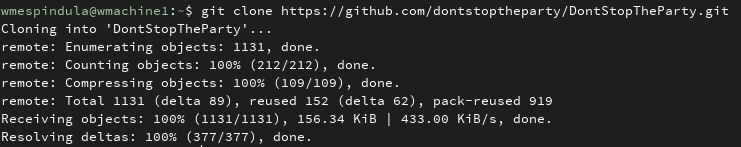
\includegraphics[width=\textwidth]{1a.png}
                \caption{Clone do Repositório. Fonte: O Autor, 2021.}
              \label{fig:question1a}
          \end{figure}
          \begin{figure}[!ht]
              \centering
              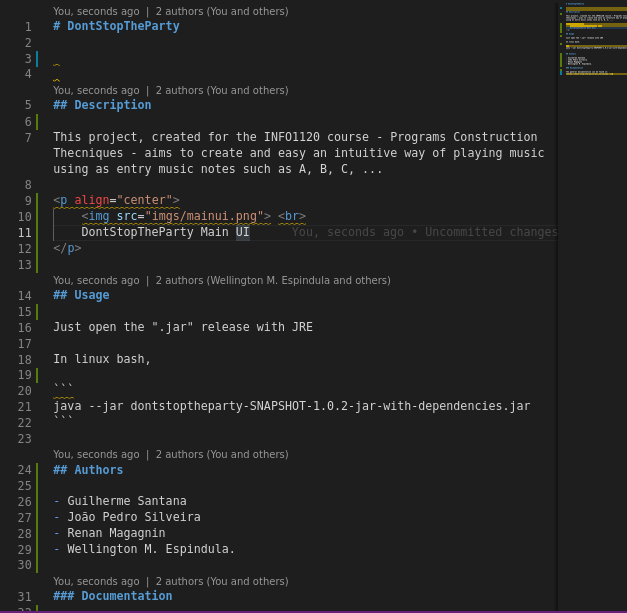
\includegraphics[width=0.7\textwidth]{1c.png}
                \caption{Alterações no README.md. Fonte: O Autor, 2021.}
              \label{fig:question1b}
          \end{figure}
          \begin{figure}[!ht]
              \centering
              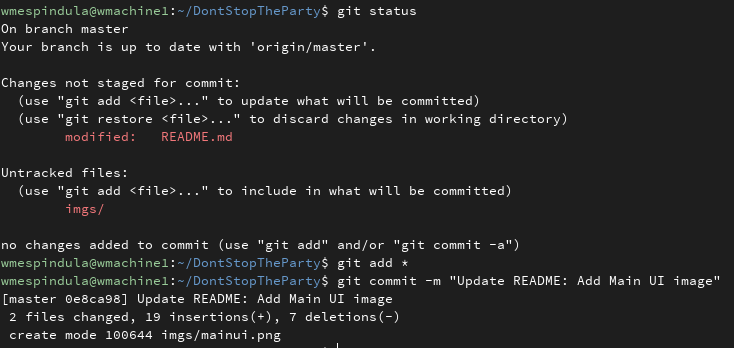
\includegraphics[width=\textwidth]{1b.png}
                \caption{Status, stash e commit das alterações. Fonte: O Autor, 2021.}
              \label{fig:question1c}
          \end{figure}
        } \clearpage
        
        % Question 2
        \question{O que é débito técnico? Quais as consequências de não considerar o gerenciamento de débito técnico em um projeto de software?}
        \answer{
            Muitas vezes no decorrer de um projeto, por diversos motivos - tais como pressão do cronograma ou falta de conhecimento -, soluções precárias - ou soluções não ótimas - acabam sendo entregues. Quando isso acontece, é denominado débito técnico, dado que é como se o projeto debitasse por um tempo aquele \quotes{problema} - solução pouco adequada e afins. Dessa forma, quanto mais tempo essa solução permanece, maior o valor a ser pago para que isso seja resolvido (juros). O exemplo mais claro é quando se realizam implementações ruins em código, como trechos de código pouco legíveis, código duplicado, code smells, entre outros. Mas de forma similar o débito técnico pode ser encontrado em diversos processos do projeto e desenvolvimento de software, existindo também o "Débito de Projeto e Arquitetura", "Débito de Documentação" e "Débito de Testes". \\
            Por conseguinte, sabendo que existe um juros ligado ao débito técnico, a falta de gestão deste débito pode levar até o projeto à "falência", dado que é necessário refatorar constantemente e pagar esse débito o mais rápido possível. Como desenvolvedor, cotidianamente, noto no projeto que participo alguns débitos técnicos de anos e como isso tem prejudicado o meu processo de desenvolvimento do software, dado que eventualmente tenho que gastar muito tempo de trabalho redesenhando essas soluções que foram pouco refatoradas - muitas vezes só foram aglutinadas outras soluções - para ser possível dar prosseguimento ao processo de desenvolvimento. Portanto, sabendo que existe um débito técnico no processo de desenvolvimento, faz-se necessário tentar gerir o mesmo a fim de reduzir os danos gerados por estes.  
        } \newpage
        
        % Question 3
        \question{Escolha um padrão de projeto GoF não apresentado em aula. Escreva um pequeno código que ilustre o seu uso. Faça o diagrama de classes e de sequência que represente este código e coloque no relatório. }
        \answer{
            Quando se trata de realizar ações, um padrão muito útil é o \tit{Command}, também conhecido por \tit{Action} ou  \tit{Transaction}. A principal ideia deste padrão é encapsular uma solicitação em um objeto. Isso torna possível parametrizar diferentes solicitações, enfileirar ou registrar (\tit{logging}), além de suportar o desfazer das operações e a estruturação um sistema sobre operações de alto nível construídas em cima de operações primitivas. Para título de exemplo, nas figuras \ref{fig:question3a} e \ref{fig:question3b}, utilizei o padrão \tit{Command} para comandos de Banco de Dados. Para tanto, os comandos de banco de dados irão realizar chamadas assíncronas. Dessa forma, na figura \ref{fig:question3a}, pode-se notar que um comando de banco de dados (\tit{DbCommand}) seria composto, de forma simples, de um comando de execução (\tit{execute()}) e de um comando de desafazer (\tit{rollback()}). \\
            Para exemplificar o uso deste padrão, eu criei uma gerenciadora do fluxo de transações em Banco de Dados (\tit{DatabaseAdministrator}) responsável por gerenciar uma fila de solicitações de Comandos. Na classe \tit{Main}, simulando um cliente qualquer, eu consumi o \tit{DatabaseAdministrator}. Da mesma forma que utilizei esse administrador de banco de dados para o exemplo do uso do \tit{Command}, eu poderia ter utilizado classes \tit{DAO} fazendo uso desses comandos. \\
            Desta forma, o Gerenciado de Banco consegue utilizar os Comandos encapsulados como objetos, salvando um histórico de usos e possibilitando o rollback quando necessário. Ademais, o padrão \tit{Command} permite que um comando tenha uma vida independente da solicitação original. Pensando nisso, tentei exemplificar tendo em vista que os comandos de banco de dados podem ser assíncronos e o \tit{DbCommandStateChangedReceiver} irá informar quando a solicitação foi concluída. \\
            O código-fonte deste exemplo foi disponibilizado em \url{https://github.com/WellingtonEspindula/INF01127-CommandExample}.
        }
        
        \clearpage
        \begin{lstlisting}
                    public class Main {

                        public static void main(String[] args) {
                    	    DatabaseAdministrator dbAdmin = new DatabaseAdministrator();
                    	    dbAdmin.enqueue(new InsertionDbCommand("mTable", new HashMap<>(){{
                    	        put("id", "001");
                    	        put("name", "Wellington Espindula");
                    	        put("telephone", "+5551000000000");
                            }}));
                    
                    	    dbAdmin.start();
                    
                    	    dbAdmin.enqueue(new InsertionDbCommand("mTable", new HashMap<>(){{
                    	        put("id", "002");
                    	        put("name", "Fulano Espindula");
                    	        put("telephone", "+5551000000000");
                            }}));
                    
                    	    dbAdmin.enqueue(new InsertionDbCommand("mTable", new HashMap<>(){{
                                put("id", "003");
                    	        put("name", "Fulano Ciclano");
                    	        put("telephone", "+5551000000000");
                            }}));
                    
                    	    dbAdmin.enqueue(new UpdateDbCommand("mTable", "003", new HashMap<>(){{
                    	        put("name", "Fulano Ciclano da Silva");
                    	        put("telephone", "+55510000000012");
                            }}));
                        }
                    }
        \end{lstlisting}
        \newpage
        \begin{lstlisting}
                    public class DatabaseAdministrator implements Runnable {
                
                    private boolean isRunning;
                    private boolean currentCommandIsFinished;
                    private List<DbCommand> history;
                    private Queue<DbCommand> operationsQueue;
                
                    private final DbCommandStateChangedReceiver dbCommandStateChangedReceiver = newState -> {
                        if (newState == DbCommandState.FINISHED){
                            finishedCurrentCommand();
                        }
                    };
                
                    public DatabaseAdministrator() {
                        isRunning = false;
                        history = new ArrayList<>();
                        operationsQueue = new LinkedList<>();
                        currentCommandIsFinished = false;
                    }
                
                    public void start() {
                        isRunning = true;
                        Thread newThread = new Thread(this);
                        newThread.start();
                
                    }
                
                    public void stop() {
                        isRunning = false;
                    }
                
                    private void finishedCurrentCommand() {
                        currentCommandIsFinished = true;
                    }
                
                    public void enqueue(DbCommand command){
                        command.setReceiver(dbCommandStateChangedReceiver);
                        operationsQueue.add(command);
                    }
                
                    public List<DbCommand> getHistory(){
                        return history;
                    }
                
                    @Override
                    public void run() {
                        while (isRunning) {
                            // Supressed
                        }
                    }
                }
            \end{lstlisting}
        
        
         \begin{figure}[!ht]
              \centering
              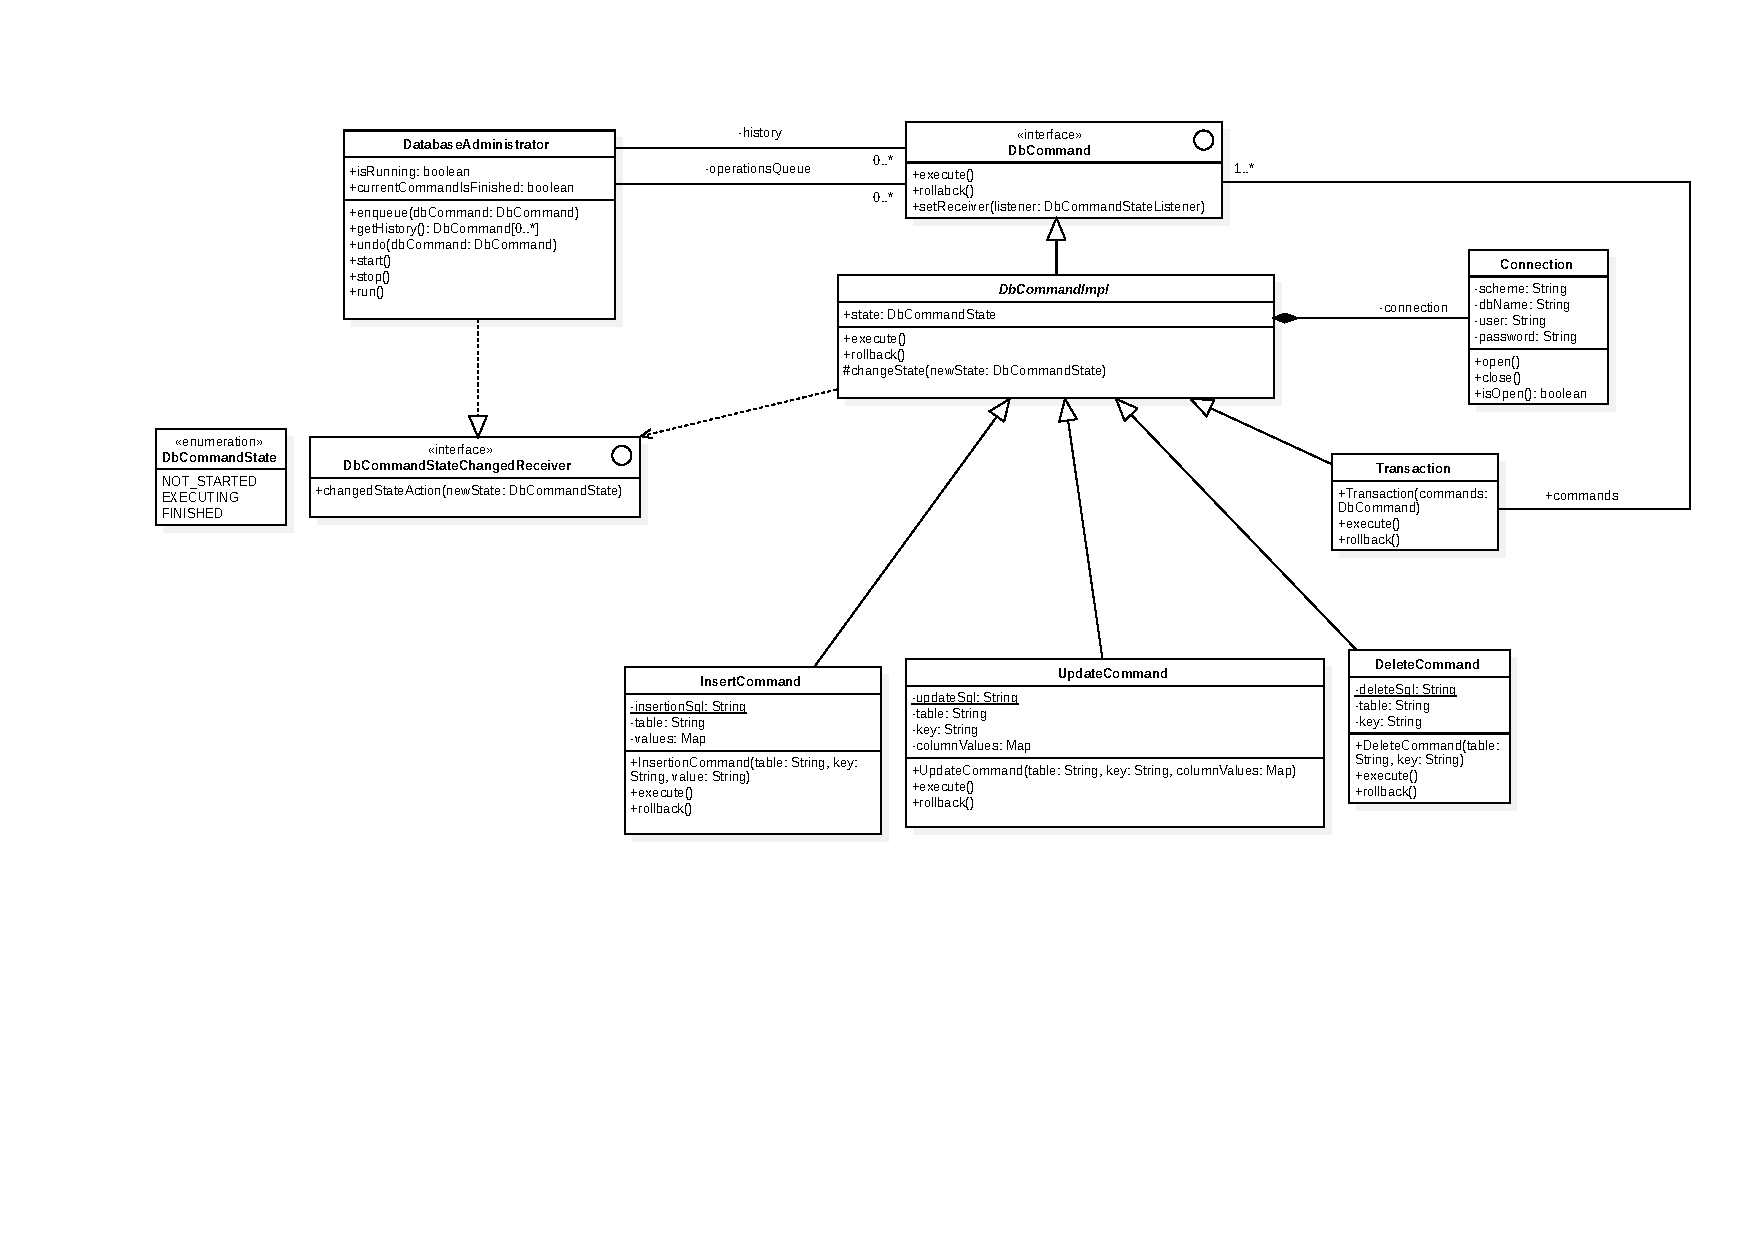
\includegraphics[width=\textwidth, trim = 2cm 6cm 1cm 1cm, clip]{3a.pdf}
                \caption{Exemplo de Diagrama de Classes do padrão \tit{Command}. Fonte: O Autor, 2021.}
              \label{fig:question3a}
          \end{figure}
          
           \begin{figure}[!ht]
              \centering
              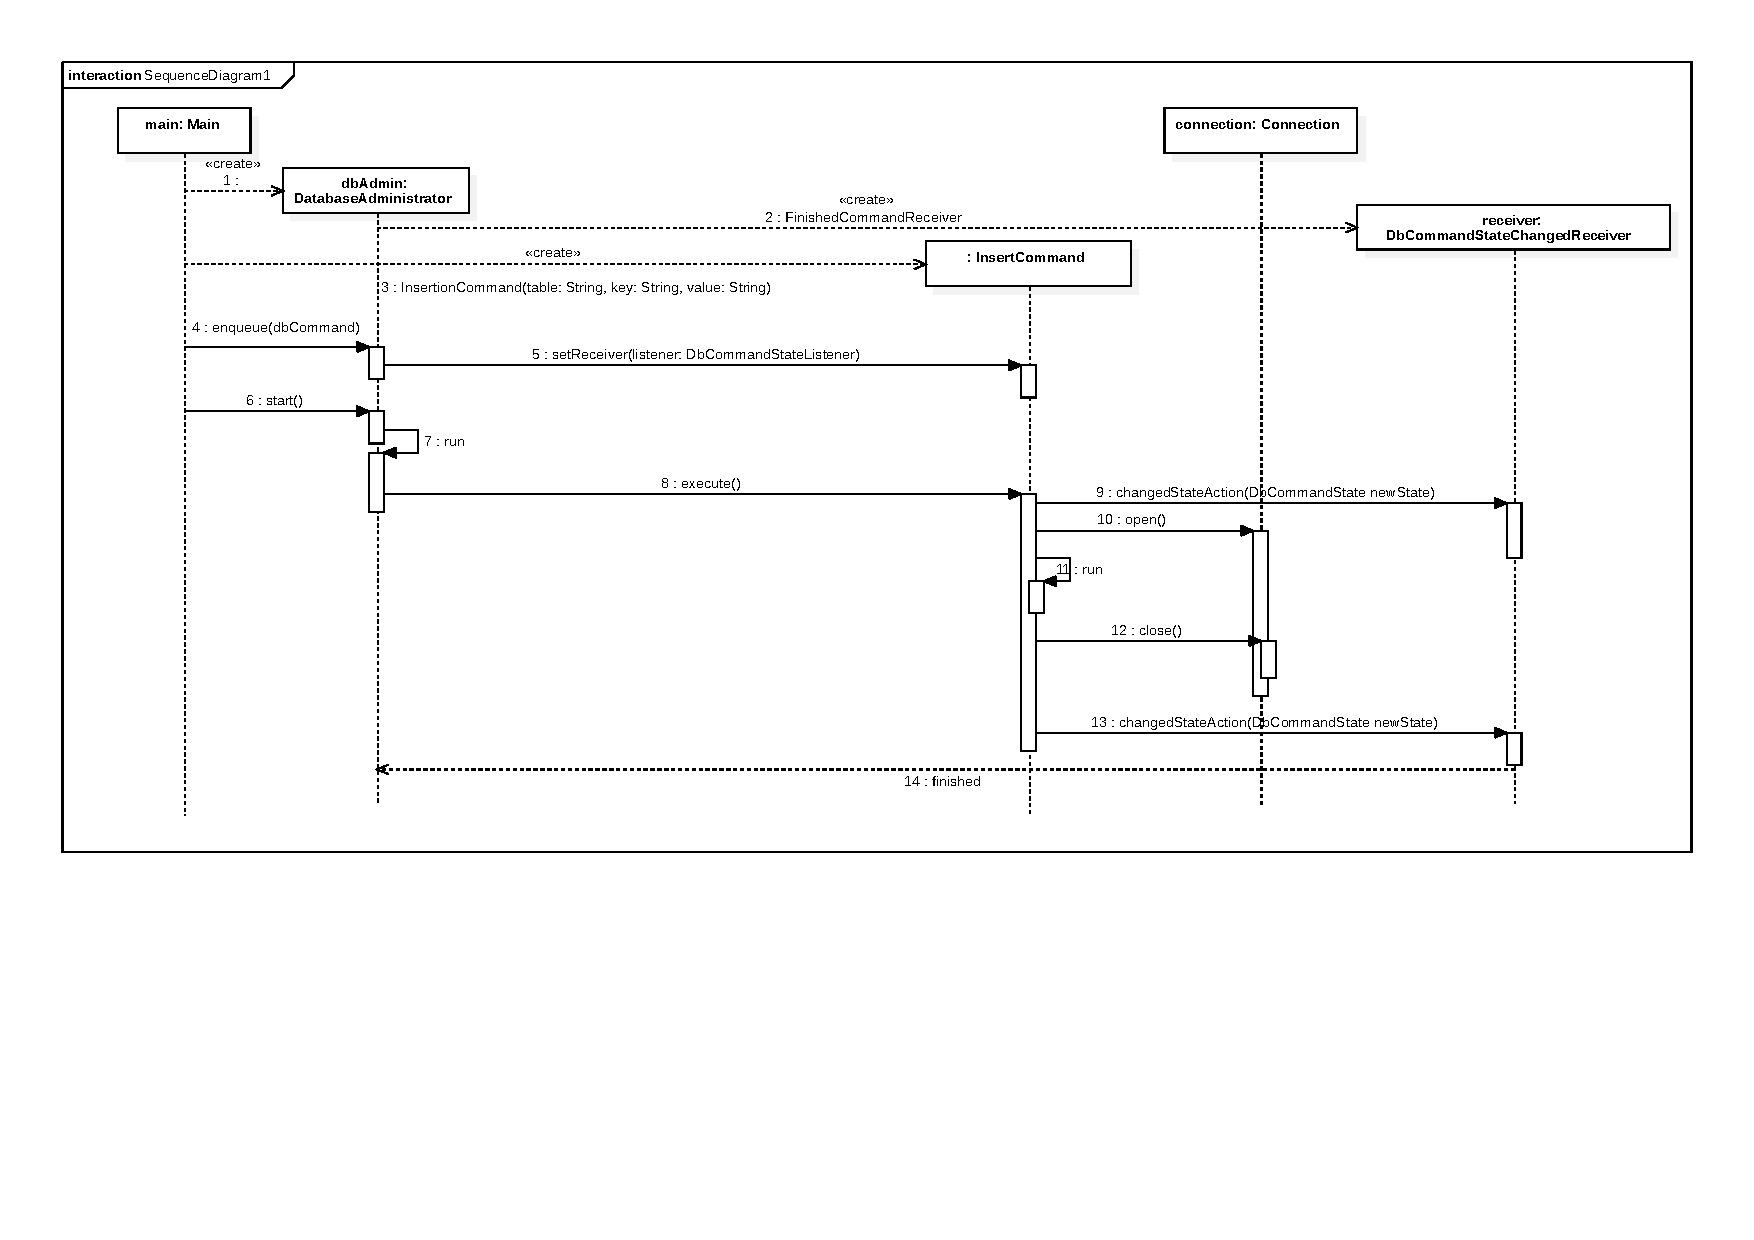
\includegraphics[width=\textwidth, trim = 1cm 6cm 1cm 1cm, clip]{3b.pdf}
                \caption{Exemplo de Diagrama de Sequência do padrão \tit{Command}. Fonte: O Autor, 2021.}
              \label{fig:question3b}
          \end{figure}
        % \newpage
        
        \clearpage
        \newcommand{\fw}{\tit{framework} }
        \newcommand{\fws}{\tit{frameworks} }
        % Question 4
        \question{Faça um resumo (cerca de meia página) sobre \fws, desenvolvimento baseado em componentes e linhas de produto de software. Explique o que são cada uma dessas formas de reuso, como o reuso é realizado, quais suas vantagens e quais são os seus riscos.}
        \answer{ 
            Os \tit{Frameworks} são largamente utilizados pela indústria de software, existindo diversos tipos para diversas finalidades em diferentes linguagens de programação. Os \fws fornecem um tipo de \tb{reuso para os clientes através da inversão de controle}. Na prática, isso significa que os clientes irão estender os componentes do \fws ao invés de fazer chamadas diretas - como ocorre no uso de bibliotecas -, fazendo que o \fw retenha o fluxo de controle do software e realize as chamadas de componentes. Assim os \fws geram determinados pontos de extensão (\tit{hot-spots}) em que o cliente conecta suas partes com suas devidas particularidades. Esses pontos de extensão podem ser \iitem{i} \tb{white-box}: por herança direta de uma classe abstrata; \iitem{ii} \tb{black-box}: realizam-se configurações através de arquivos de configuração (xml, yaml, etc) ou por wizard; e \iitem{iii} \tb{gray-box}: envolve ambas composição (herança) e configuração. Por conseguinte, os \fws maximizam o reuso, a confiabilidade, diminuem a quantidade de manutenção, tornam o código mais conciso e mais consistente. Em contrapartida, a eficiência pode ficar comprometida dada a quantidade de flexibilidade e generalizações. A nível de desenvolvimento do \tit{framework}, o seu próprio desenvolvimento é difícil, juntamente com sua documentação a manutenção a fim de mantê-lo retro-compatível com versões anteriores.  \\
            O Desenvolvimento Baseado em Componentes (CBSE) realiza basicamente no \tb{reuso mais tradicional e efetivo de utilizar componentes prontos acessando-os através de suas interfaces (cada componente tem uma interface provida e requerida)}. Portanto, o desenvolvimento é baseado em componentes independentes entre si, altamente coesos, com implementação escondida e interfaces bem definidas. Para tanto, é necessário ter confiança nos componentes utilizados e não existe necessariamente uma análise de certificação destes. Assim, muitas vezes tem de se fazer uma análise de trade-offs comparando as características de componentes a fim de encontrar o que atende melhor aos requisitos esperados. \\
            Por fim, as linhas de produto é uma forma de desenvolvimento que faz alusão à linha de produção de um carro; sendo assim, a ideia base da linhas de produto é \tb{realizar o desenvolvimento de software utilizando a mesma arquitetura para diversos softwares} com o mesmo propósito e alterando as \tit{constraints} para cada um dos softwares entregues conforme as demandas dos clientes. A maior desvantagem é que existe alta demanda do tempo no início do processo de criação e desenvolvimento da linha de produtos. Em contrapartida, assim que está no mercado, reduz-se o custo de desenvolvimento e manutenção bem como o tempo para tal.
        }
        % \newpage
        
         % Question 5
        \question{Qual o \fw que realiza a injeção de dependência no estudo de caso da Biblioteca?}
        \answer{ 
            O \fw que realiza a injeção de dependência no sistema Biblioteca é o \tit{Spring}. Dadas os módulos e outras configurações declaradas nas configurações do \tit{Spring}, ele atuará nesse sistema orquestrando os módulos de forma a instanciá-los e injetá-los como parâmetros nos objetos dependentes deste.
        }     
    
    \end{enumerate}
        
    
\end{document}